%!TEX root = 16-ra-letter-NMPCWalkGen.tex

In the present chapter we present a real-time nonlinear model predictive control (NMPC) executable on the humanoid robot HRP-2.
This chapter has been developed in the frame of the collaborative project \koroibot\ and published in \cite{naveau:ral:2016}.
Following the idea of ``walking without thinking", we propose a walking pattern generator that takes into account simultaneously the position and orientation of the feet.
A requirement for an application in real-world scenarios is the avoidance of obstacles.
Therefore, an extension of the pattern generator that directly considers the avoidance of obstacles is derived.
The algorithm uses the whole-body dynamics to correct the center of mass trajectory of the underlying simplified model.
The pattern generator runs in real-time on the embedded hardware of the humanoid robot HRP-2 and experiments demonstrate the increase in performance with the correction.

In Sec.~\ref{Sec:nmpcmotivation} we present the motivation and the related works. Sec.~\ref{Sec:dynamic} is a reminder of the LIPM equation as well as the principles used in \cite{herdt:iros:2010}. Sec.~\ref{Sec:nmpc} depicts the formulation of the problem as a sequence of locally linearized quadratic problems and the real-time feasible solution by applying the idea of the so called "real-time" iteration.
A particular treatment of the dynamical filter is given in Sec.~\ref{Sec:dynamic_filter}.
Finally, our practical contribution, showing that the algorithm can be implemented in real-time on the humanoid robot HRP-2, is detailed in Sec.~\ref{sec:experiments_with_hrp2}.

\section{Introduction}

\subsection{Motivation}
\label{Sec:nmpcmotivation}

The recent DARPA robotics challenge have shown the need for humanoid robots with an increased level of functionality
enabled by proper control.
Such complex robots must provide a simple interface for humans and handle as much as possible the motion generation autonomously.
A general scheme is to use a motion planner to find an optimal path over a discrete set of foot-step transitions between two quasi-static poses \cite{Chestnutt:2010:MPHR,Hornung:ICHR:12}.
The foot-steps transition are given by a statistical exploration of a whole-body controller together with a walking pattern generator.
The planner then finds a feasible sequence of quasi-static poses and foot-step transitions which minimizes a cost function and avoids obstacles.
This solution is then improved online while ensuring feasibility, see for instance \cite{perrin:itro:12}.
In general it is not possible to realize real-time motion planning by directly using the controller itself because it is not possible to run more than one or two instances of the same controller before collision.
Therefore, when the planner fails it is necessary to solve a continuous local problem which will provide a feasible solution different from the precomputed one \cite{Chestnutt:2010:MPHR}.
The statistical exploration can be advantageously used to cast an optimization problem to find an initial guess \cite{Chestnutt:2010:MPHR}.
Recently, \emph{Deits} proposed to define the area of convergence for a local convex problem with linear constraints \cite{deits:ichr:14}
for a template model.
With template models the inertia related to the whole-body motion is ignored, regulated to zero or corrected.
In this chapter it is corrected by means of a dynamic filter. It is shown in the experimental section that it is drastically improving the 
performances over \cite{herdt:iros:2010} on the same robot.
The use of template model is a practical solution on platforms with limited computation capabilities.
%\todo{%
Even if advanced whole-body motion controllers are now closer to real-time feasibility, e.g. the one proposed by \emph{Todorov} which was recently applied to
HRP-2~\cite{Koenemann:iros:2015}, they still need powerful multi-core CPUs which limit their integration on humanoid robots due to heat and power consumption.
\begin{figure}[t]
  \centering
  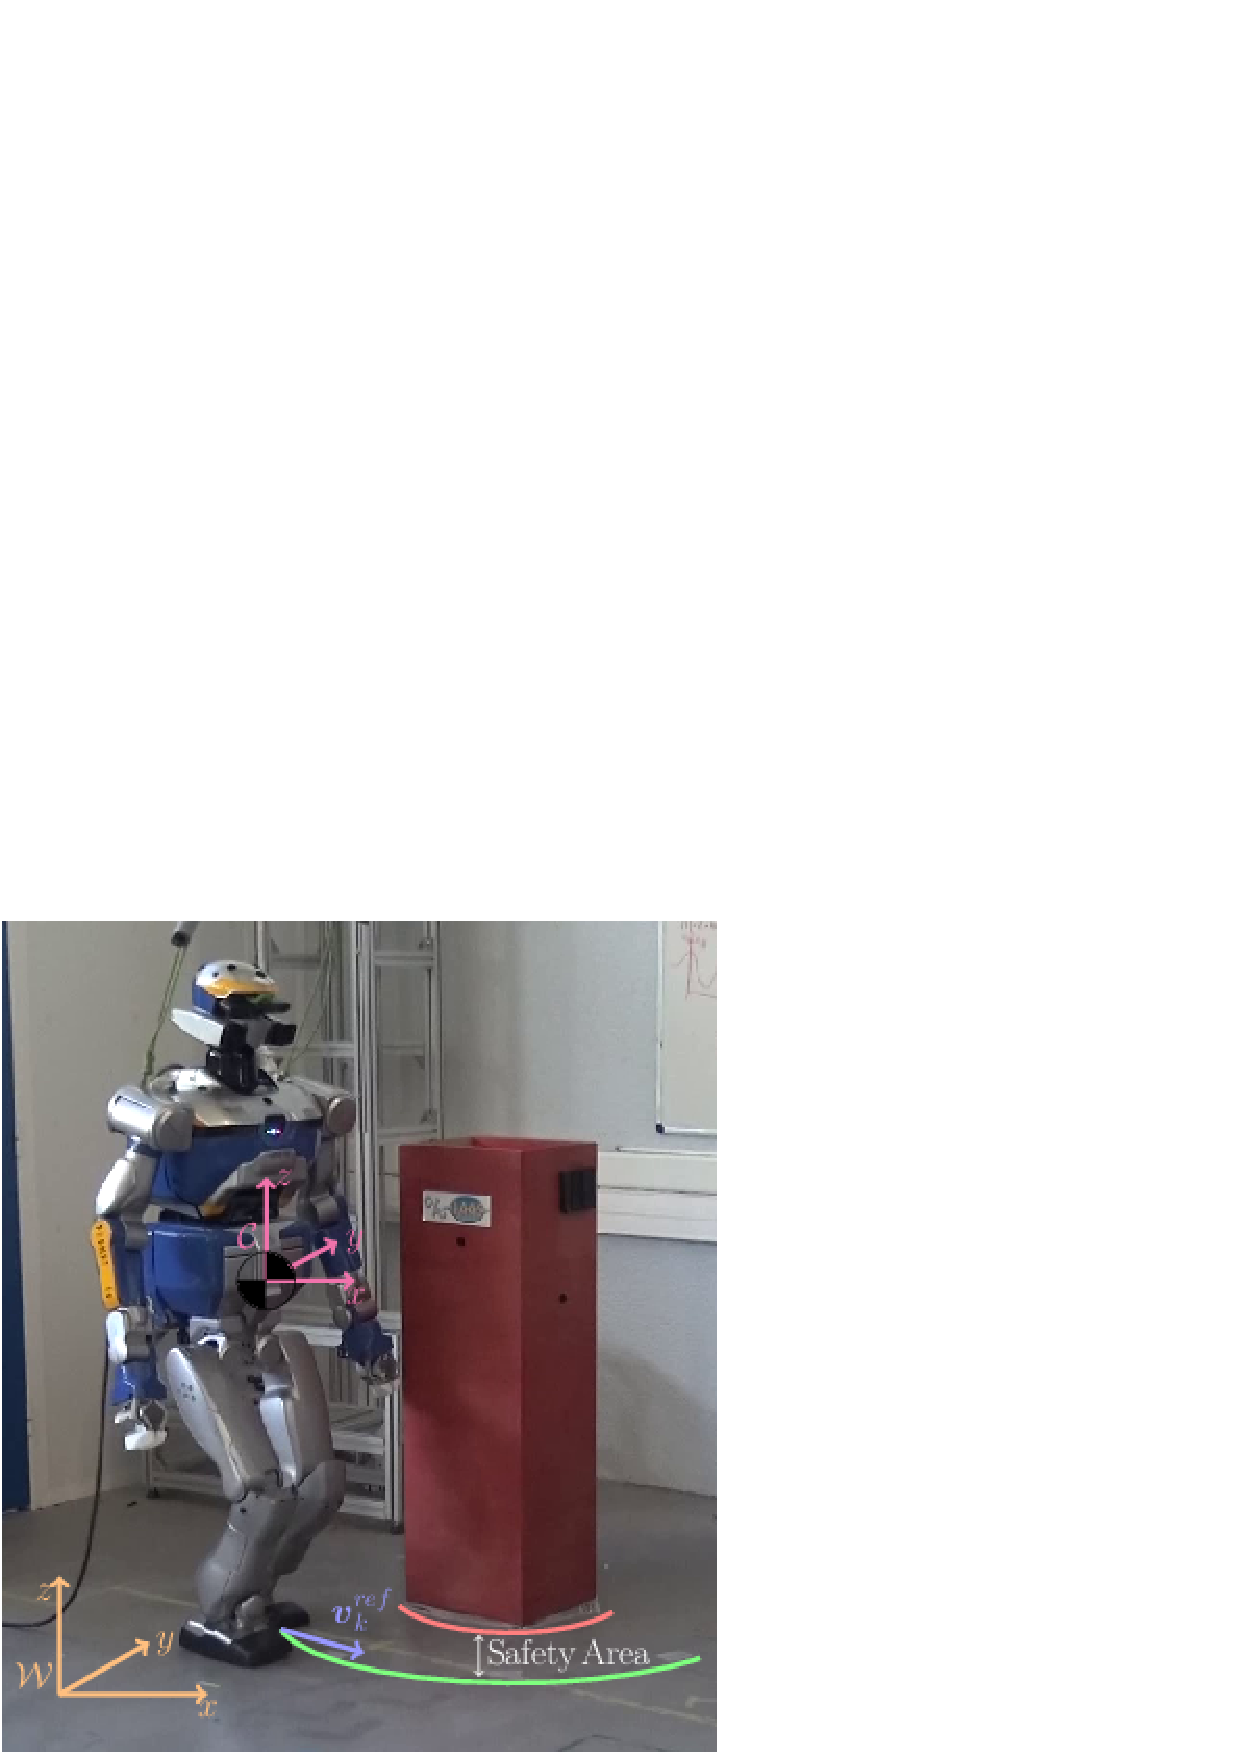
\includegraphics[width=0.4\linewidth, keepaspectratio]{synthesis.pdf}
  \caption[Problem setup]{HRP-2 avoiding reactively on an obstacle, even if the reference velocity $v^{ref}_k$ drives it into it. The upper body geometry is taken into account by setting a constraint (in green) such that the robot is sufficiently away from the obstacle (in red).}
  \label{fig:covernmpcwalkgen}
\end{figure}

Another improvement of this chapter over the method developed in \cite{herdt:iros:2010} is the nonlinear formulation which here allows to deal with obstacle.
More precisely \cite{herdt:iros:2010} integrates the information provided by statistical exploration of the controller feasibility 
between two foot-step transitions. It makes possible to correct foot-steps while having a guarantee over their feasibility.
%directly inside the walking pattern generator and is able to correct foot-steps. (MK: where is statistical exploration in the PG. Can you clarify? Is it a combination of planning and motion generation that you mean?)
%}
It is realized by reformulating the optimization problem to generate balanced Center-of-Pressure (CoP) and Center-of-Mass (CoM) trajectories where the free variables are the jerk of the CoM as well as foot-step positions and orientations.
The feasible foot-steps, i.e. free of self-collision and singularities, are specified through linear constraints.
This works well for level ground walking, unfortunately integrating obstacles with linear constraints implies a pre-processing of the environment or to use a different solver.

The present chapter shows that obstacles can be dealt with in real-time using a nonlinear scheme.
Although not demonstrated in this chapter, it can be coupled with a real-time planner.
The proposed method would provide a local feasible solution while the planner is looking for a global feasible solution \cite{perrin:itro:12}.
%For this reason, approaches with simple user input, e.g. the direction of walking and average velocity, have a high potential regarding real-world applications.
%This requires the robot to be able to find its foot steps and provide stability while walking autonomously.
%\todo{Furthermore, a highly capable controller lowers the burden of motion planners (MK: Do we use that?)}.

\subsection{Related work}
Previous works have proposed to apply Model Predictive Control (MPC) to humanoid robots walking by considering either the whole body or a template model.
When a model is available for a robot, MPC has several advantages.
It can be very fast when using analytical solutions \cite{Morisawa:ICRA:2007,Tedrake:ur:15,Faraji:ICRA:2014}.
However such formulation makes generally some specific assumptions to find the derivation.
This makes difficult the extension to other walking functionalities.
On the other hand 
MPC schemes formulated as an optimization problem  with a finer discretization grid can be more easily modified to include various walking modes 
inside a single formulation \cite{Sherikov:ichr:2014}.
In addition MPC as an optimization problem is becoming increasingly popular \cite{Feng:ichr:2013}, 
because for a given class of problems it allows using efficient off-the-shelf solvers.
Moreover several methods exist to increase the efficiency of solvers for NMPC problems.
For instance, it is possible to use warm-starts or use a sub-optimal solution while maintaining feasibility \cite{Boyd:CO:2004}.
The goal in humanoid robotics is to find a problem formulation which realizes all the needed functionalities and copes with the robot capabilities.
The locomotion problems described in \cite{mordatch:tog:12}, that include multi-contacts and consider the whole robot model over a time horizon, 
are not yet solvable in real-time and strongly depend on the models used to represent the physics.

Despite numerous efforts to address this large scale nonlinear problem with roughly ten thousand variables \cite{Koenemann:iros:2015,Dai:ICHR:2014}, no solution yet exists to generate physically consistent controls in real-time using humanoid robot embedded computers.
On the other hand template models projecting the overall robot dynamics to its CoM are used in research works \cite{Wensing:iros:2014,Orin:AURO:2012,Kajita:icra:2003,Englsberger:ichr:2015}, and already showing promising performance.
Motion generation with template models can sometimes be solved analytically, and in such cases provide fast solutions that are particularly well suited for platforms with limited computational power.
However, when increased CPU power is available, MPC-based solutions with the whole model are much more complete and reliable.
Furthermore, as they can be easily modified, they provide more adaptive functionalities.
In this chapter, with a bottom-up approach, we are trying to increase the functional level of a control architecture that already works on an existing humanoid robot, HRP-2 \cite{herdt:iros:2010}.
The point of this chapter is to present extensions of the linear MPC scheme presented in \cite{herdt:iros:2010}, that allows automatic foot placement in real-time.
For instance, the problem depicted in Fig.~\ref{fig:covernmpcwalkgen} shows the humanoid robot HRP-2 driven by a desired velocity provided by the user.
%\todo{%
The former scheme \cite{herdt:iros:2010} was specifically formulated as a cascade of two quadratic programs (QPs). Foot-step orientations are solution of the first problem, while the second solution of the second QP provides the CoM trajectory and foot-step positions. This separation is efficient because the constraints are linear.
%(say something about position and orientation?)}
If an obstacle has to be taken into account then the constraints have the shape depicted in Fig.~\ref{fig:algo_diff}, which is not convex anymore.
To maintain the convexity, the solution would be to pre-process the obstacle and the feasibility area of the foot-steps.
However a linearization of the obstacle boundary is equivalent to adding a linear constraint as depicted in Fig.~\ref{fig:algo_diff}.
The algorithm proposed in this chapter is doing a similar operation and therefore no pre-processing is necessary.
This is one of the major contribution of this chapter in comparison to \cite{herdt:iros:2010}.
The proposed nonlinear extension takes into account the exact expression of constraints such as, for instance, locally avoiding a convex obstacle.
Other formulations for walking motion generation have already been proposed.
\cite{deits:ichr:14} is using mixed-integer convex optimization for planning foot-steps with Atlas.
\cite{Ibanez:ark:14} is using mixed-integer convex optimization for MPC control and foot steps timing.
In this work we introduce three nonlinear inequalities to handle balance, foot step orientation and obstacle avoidance.
This new real time walking pattern generator has been successfully tested on the humanoid robot HRP-2 as depicted in Fig.~\ref{fig:covernmpcwalkgen}.
A key ingredient for achieving real-time performance was the following observation: \emph{one real-time iteration of the nonlinear scheme is enough to find a reasonable solution}.

\begin{figure}[ht]
    \centering
    %!TEX root = ../../14-icra-RealTimeNMPC.tex

\newcommand{\tetazero}{20.55}
\newcommand{\Fkxzero}{-20}
\newcommand{\Fkyzero}{20}

\newcommand{\tetaone}{-20}
\newcommand{\Fkxone}{5}
\newcommand{\Fkyone}{0}

\newcommand{\tetatwo}{20}
\newcommand{\Fkxtwo}{25}
\newcommand{\Fkytwo}{20}

%\includegraphics[width=15cm]{./figures/walking-without-thinking/ConvexHull}
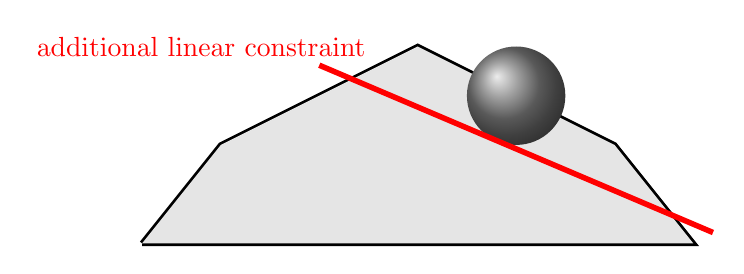
\begin{tikzpicture}[scale=0.125]
%\draw [dashed][->](-50,0) -- (50,0) node [below left, black]{$\overrightarrow{x}$}; %x-axis
%\draw [dashed][->](0,-50) -- (0,50) node [below left, black]{$\overrightarrow{y}$}; %y-axis
 %left support, right foot landing convexhull
\draw [line width=2pt](-28,20)--(-20,30)--(0,40)--(20,30)--(28,20)--(-28,20) node at (-10,30)[black]{} ;
\fill [color=gray!20,line width=2pt] (-28,20)--(-20,30)--(0,40)--(20,30)--(28,20)--(-28,20) ;
%pattern=north east lines
 %support foot
%\draw (-10,-5)--(10,-5)--(10,5)--(-10,5)--(-10,-5) node [below left, black]{Support Foot} ;

\shade[ball color=gray] (10,35) circle (5cm);

\draw [line width=2pt,red](-10,38.10)--(30,21.10) node at (-22,40)[red]{additional linear constraint} ;
\end{tikzpicture}

%
%\begin{tikzpicture}[x=0.7cm,y=0.7cm]
%\node (D) at (0,0) [coordinate] {} ;
%\node [below left] at (D) {D} ;
%\node (G) at (3,0) [coordinate] {} ;
%\node [below] at (G) {G} ;
%\node (C) at (5,0) [coordinate] {} ;
%\node [below right] at (C) {C} ;
%\node (F) at (5,3) [coordinate] {} ;
%\node [right] at (F) {F} ;
%\node (B) at (5,5) [coordinate] {} ;
%\node [above right] at (B) {B} ;
%\node (E) at (2,5) [coordinate] {} ;
%\node [above] at (E) {E} ;
%\node (A) at (0,5) [coordinate] {} ;
%\node [above left] at (A) {A} ;
%\node (H) at (0,2) [coordinate] {} ;
%\node [left] at (H) {H} ;
%\filldraw[color=lightgray] (D) -- (G) -- (H) ;
%\filldraw[color=lightgray] (G) -- (C) -- (F) ;
%\filldraw[color=lightgray] (F) -- (B) -- (E) ;
%\filldraw[color=lightgray] (E) -- (A) -- (H) ;
%\draw (D) -- node[below] {$b$} (G) -- node[below] {$a$} (C) ;
%\draw (C) -- node[right] {$b$} (F) -- node[right] {$a$} (B) ;
%\draw (B) -- node[above] {$b$} (E) -- node[above] {$a$} (A) ;
%\draw (A) -- node[left] {$b$} (H) -- node[left] {$a$} (D) ;
%\draw (G) -- (F) ;
%\draw (F) -- (E) ;
%\draw (E) -- (H) ;
%\draw (H) -- (G) ;
%\end{tikzpicture}
%
%
%
%
%\begin{tikzpicture}[x=0.7cm,y=0.7cm]
%\node (D) at (0,0) [coordinate] {} ;
%\node [below left] at (D) {D} ;
%\node (G) at (3,0) [coordinate] {} ;
%\node [below] at (G) {G} ;
%\node (C) at (5,0) [coordinate] {} ;
%\node [below right] at (C) {C} ;
%\node (F) at (5,3) [coordinate] {} ;
%\node [right] at (F) {F} ;
%\node (B) at (5,5) [coordinate] {} ;
%\node [above right] at (B) {B} ;
%\node (E) at (2,5) [coordinate] {} ;
%\node [above] at (E) {E} ;
%\node (A) at (0,5) [coordinate] {} ;
%\node [above left] at (A) {A} ;
%\node (H) at (0,2) [coordinate] {} ;
%\node [left] at (H) {H} ;
%
%\filldraw[color=lightgray,pattern=crosshatch] (G) -- (C) -- (F) ;
%\filldraw[color=lightgray,pattern=crosshatch] (F) -- (B) -- (E) ;
%\filldraw[color=lightgray,pattern=crosshatch] (E) -- (A) -- (H) ;
%\draw (D) -- node[below] {$b$} (G) -- node[below] {$a$} (C) ;
%\draw (C) -- node[right] {$b$} (F) -- node[right] {$a$} (B) ;
%\draw (B) -- node[above] {$b$} (E) -- node[above] {$a$} (A) ;
%\draw (A) -- node[left] {$b$} (H) -- node[left] {$a$} (D) ;
%\draw (G) -- (F) ;
%\draw (F) -- (E) ;
%\draw (E) -- (H) ;
%\draw (H) -- (G) ;
%\end{tikzpicture}

    \caption{Walkable zone distorted by a convex obstacle}
    \label{fig:algo_diff}
\end{figure}

\subsection{Contribution of the chapter}

%\textcolor{blue!70}{The contributions of this work are the following:
\begin{itemize}
\item It proposes a nonlinear reformulation of classical walking pattern generator able to find simultaneously foot-step positions and orientations.
\item It introduces nonlinear constraints able to cope with obstacles in the environment.
\item It shows experimentally that one iteration of the nonlinear iterative scheme provides a suboptimal but sufficient solution for practical cases.
\item Thanks to the use of a dynamical filter that corrects the CoM trajectory to compensate the limitation of the template model as in \cite{Nishiwaki:IJRR:09}
the whole body dynamics can be taken into account. This technical implementation has a strong impact on the robot performances.
\item The whole algorithm runs in real time on the embedded hardware of the human-size humanoid robot HRP-2.
\end{itemize}
To be completely fair we are not doing NMPC using sensor feedback on the walking pattern generator.
The feedback loop of the algorithm is done by the dynamic filter (see Fig.~\ref{fig:combined_feedback_scheme}).
In fact the sensor feedback is already done by the commercial stabilizer from Kawada Industry.
Additional ongoing work is done to close the loop but the stabilizer is a closed-source software.
Hence it is rather difficult to be exactly sure of its behavior.

